\chapter[Introdução]{Introdução}
%\addcontentsline{toc}{chapter}{Introdução}

\section{Contextualização}

Desde o início da civilização, o homem tem olhado para os astros buscando sinais. Alguns desses homens conseguiram desvendar esses mistérios das estrelas e desenvolveram formas de governar sua vida com base na localização dessas. Alguns dos primeiros observadores dos astros os utilizaram para determinar a passagem do tempo, marcando o intervalo transcorrido até que aquele astro voltasse a determinado ponto no céu; bem como para determinar a direção em que viajavam com seus grupos, usando constelções, como o cruzeiro do sul, para isso.

Tal necessidade de se localizar levou o homem a adotar métodos progressivamente mais elaborados e precisos de obter posicionamentos, utilizando, com o passar do tempo telescópios, instrumentos de medição  e até mesmo inserindo cálculos matemáticos em suas análises de comportamento dos astros. Porém, desde que foi possível utilizar satélites artificiais para obter esses dados, os métodos de geolocalização tomaram proporções não imaginadas por aqueles observadores que dependiam do alcance suas vistas, pois por meio desses foi possível ao homem localizar-se não apenas na porção de território em que habitava, mas localizar a si e outros em escala global. Por meio dos satélites atrificiais foi possível desenvolver sistemas de posicionamento globais. 

Deixando de ser dispositivos do tamanho de computadores disponíveis para militares, esses sistenmas de geolocalização estão, agora, disponíveis em todos os \textit{smartphones} e computadores pessoas. Além disso, por meio dos SDRs, \textit{Software Defined Radio}, é possível que a modulação de transmissão, e também a demodulação na recepção, sejam feitas por meio de um software. Dessa forma, é possível substituir vários componentes analógicos por dispositivos programáveis, o que garante mais flexibilidade e adptabilidade ao receptor de um sinal GNSS, \textit{Global Net Satellite System}, como explica \cite{MSadiku}.

Porém, mesmo com sua implementação em software, esses sistemas de geoposicionamento precisam continuar realizando tarefas que os sistemas tradicionais executavam a fim de obter o seu posicionamento em relação a um referencial, e uma dessas tarefas é o \textit{tracking}, isso é, o rastreamento dos satélites que se comunicam com esse receptor. A cadeia de recepção desses sinais é como mostrada na \textbf{figura \ref{fig:GNSS_flow_graph}}. Por meio dessa é possível perceber que após passar por um tratamento inicial, onde são resolvidos fatores como ruído e modulação, o sinal segue para um bloco de aquisição e para \textit{tracking}, e por meio desse são extraídos observáveis que permitem ao sistema estimar posição, velocidade e tempo (PVT) relacionadas ao satélite que transmite o sinal. 

%O presente projeto faz parte de um outro, desenvolvido por meio de PIBIC, que busca busca implementar o dispositivo um receptor de sinal GNSS em SDR, tal como mostrado na figura \ref{fig:GNSS_flow_graph}. Entretanto, este tem o seu escopo restrito à implementação do sistema de \textit{tracking},primeiramente de \textit{Delay Locked Loop} e em seguida de \textit{Frequency Locked Loop}.

%O presente projeto nasce da nescessidade de um PIBIC sobre técnicas de compressão e reconstrução esparsa em sinais GNSS, que visa à aquisição desse tipo de sianis utilizando SDR,. O escopo desse projeto, portanto, se restringe à implementação dos DLL e PLL presentes no \textit{tracking}. 



Assim, o presente projeto, nascido de um PIBIC sobre técnicas de compressão e reconstrução esparsa em sinais GNSS, que visa a implementar, em SDR, a cadeia de recepção de um sinal GNSS, tem o seu escopo restrito à implelementação do sistema de rastreamento para a mesma. Ao longo desse projeto serão aborados o funcionamento de sistemas de recpção de sinais GNSS, com foco no bloco de \textit{tracking} desses e, por fim, serão apresentados e discutidos resultados obtidos por meio do rastreamento utilizando máxima verossimilhança para essas estimativas.
\begin{figure}[h]
    \centering
    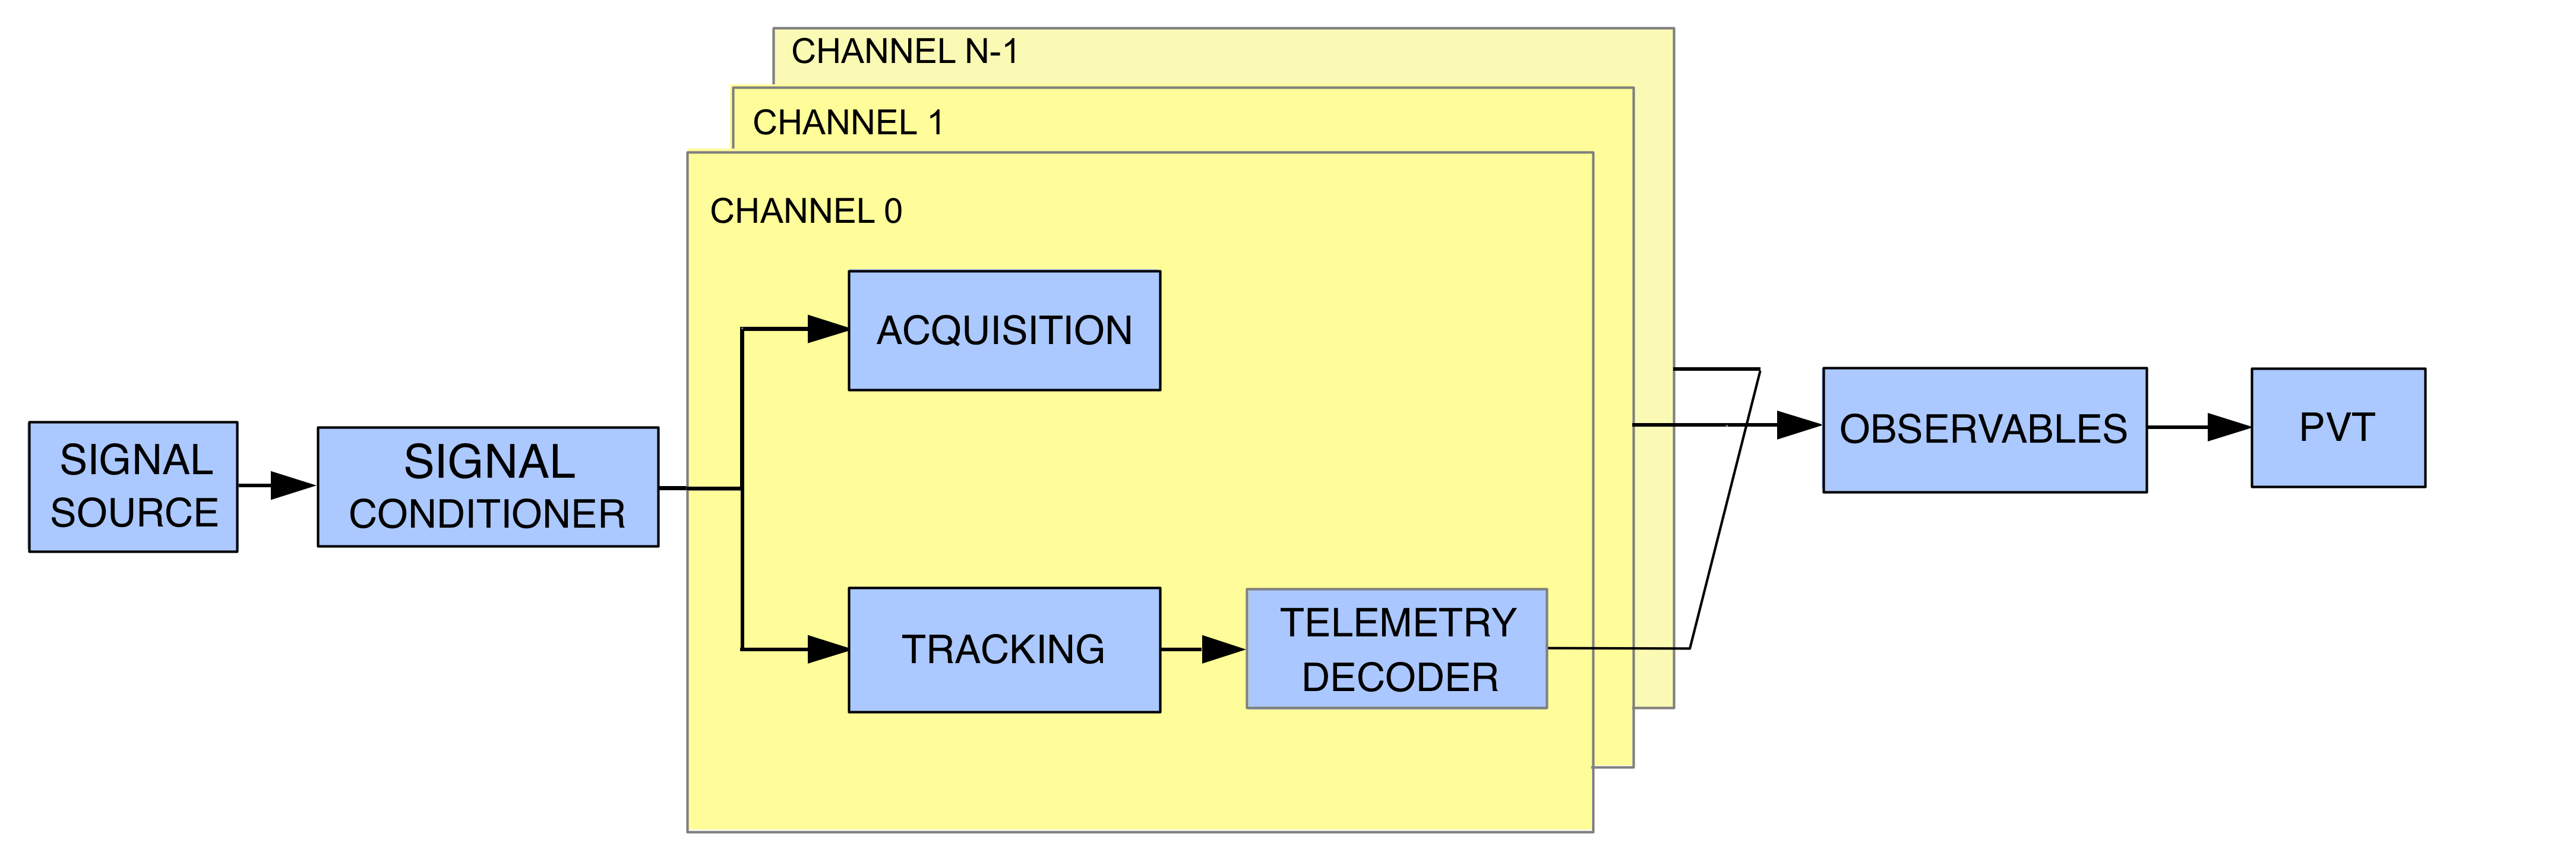
\includegraphics[width = \textwidth]{figuras/simple-gnss-sdr-flowgraph.png}
    \caption{Diagrama de blocos de receptor GNSS}
    \label{fig:GNSS_flow_graph}
\end{figure}

\section{Justificativa}

A Universidade de Brasília, no Campus Gama busca implementar um receptor se sinais GNSS. Dessa forma, surge a necessidade de se criar um recptor para esses sinais.
%Este projeto faz parte de um projeto maior desenvolvido na Universidade de Brasília, campus Gama, onde busca-se implementar todo o receptor GNSS em SDR para o laboratório de telecomunicações da universidade presente nesse campus.

%Este documento apresenta considerações gerais e preliminares relacionadas 
%à redação de relatórios de Projeto de Graduação da Faculdade UnB Gama 
%(FGA). São abordados os diferentes aspectos sobre a estrutura do trabalho, 
%uso de programas de auxilio a edição, tiragem de cópias, encadernação, etc.

%Este template é uma adaptação do ABNTeX2\footnote{\url{https://github.com/abntex/abntex2/}}.
